\documentclass[11pt,a4paper]{article}
\usepackage[margin=1in]{geometry}
\usepackage{amsmath,amssymb}
\usepackage{booktabs}
\usepackage{tikz}
\usepackage{pgfplots}
\usepackage{xcolor}
\usepackage{hyperref}
\usepackage{caption}

\pgfplotsset{compat=1.18}
\definecolor{netsogreen}{HTML}{1B4D3E}
\definecolor{netsogold}{HTML}{D4A017}

\title{\textbf{Distributed Rooftop Solar Development in Bangladesh Commercial and Industrial Facilities: Microeconomic Analysis and Financing Structures for the Netso Energy Reference Project}}
\author{\textbf{Tazwar Mahtab}\thanks{Netso Energy. Ground-truth constants generated via \texttt{System/scripts/core\_economics.py}.}}
\date{August 26, 2026}

\begin{document}

\maketitle

\begin{abstract}
Distributed commercial and industrial (C\&I) rooftop solar in Bangladesh addresses grid instability and volatile commercial utility tariffs under severe land-scarcity constraints. This paper presents the empirical and microeconomic framework of Netso Energy's reference project: an 80~kWp commercial photovoltaic installation at the Chittagong Grammar School (CGS) campus in Chattogram, Bangladesh. We evaluate operational generation physics, levelized tariff arbitrage against the Bangladesh Power Development Board (BPDB) Medium Tension category 2 (MT-2) rate, and project financing mechanisms. Operating at a 16.5\% capacity factor, the 80~kWp facility yields 115,632~kWh annually, offsetting 98.0\% of site demand. Under the baseline power purchase agreement (PPA) of BDT~10.00/kWh versus the true variable utility rate of BDT~12.98/kWh, the client achieves a 23.0\% variable expenditure savings. Under an 80/20 Infrastructure Development Company Limited (IDCOL) concessional debt structure (6.0\% p.a., 10-year amortization), the asset generates a Year-1 Debt Service Coverage Ratio (DSCR) of 2.25$\times$, an equity payback period of 1.47 years, and a 20-year levered equity internal rate of return (IRR) of 68.7\%. We examine the policy sensitivity of the FY2026--27 zero-tariff import schedule and evaluate an alternative non-dilutive 35\% gross revenue-share investment structure underwritten by Beringia Energy.
\end{abstract}

\section{Introduction}
Industrial and commercial power consumers across Bangladesh encounter rising tariff schedules, load shedding, and grid transmission congestion \cite{netso_product}. While conventional utility-scale solar farms require substantial contiguous acreage that is scarce in urbanized and agricultural regions, commercial concrete rooftops provide an unmonetized structural layer for distributed electricity generation \cite{netso_product}.

Netso Energy operates as an independent developer deploying build-own-operate (BOO) and renewable energy service company (RESCO) infrastructure. The foundational physical hardware platform comprises the Solar Pergola, an engineered modular structural canopy that provides simultaneous shading, weather shelter, and photovoltaic power generation on flat rooftops \cite{netso_product}.

To establish bankability and investor underwriting standards, Netso Energy structured an 80~kWp reference deployment at the Chittagong Grammar School (CGS) facility in Chattogram \cite{gt_constants, netso_entity}. This paper presents the end-to-end techno-economic specification, empirical utility audit analysis, financial capitalization models, and contract risk mitigations governing this reference installation.

\section{Methods}
\subsection{Physical Generation Model}
Solar photovoltaic generation is modeled using site-specific empirical solar irradiance parameters for Chattogram, Bangladesh. Annual electrical energy generation $E_1$ in kilowatt-hours (kWh) during Year~1 is governed by:
\begin{equation}
E_1 = P_{\text{dc}} \times 8760 \times \text{CF}
\label{eq:generation}
\end{equation}
where $P_{\text{dc}} = 80\text{ kWp}$ is the direct-current nameplate capacity, $8760$ represents total annual operating hours, and $\text{CF} = 0.165$ (16.5\%) is the empirical capacity factor for Chattogram \cite{gt_constants}.

Annual energy yield degrades continuously across operating lifespan $t \in [1, 20]$ at an annual degradation coefficient $\delta = 0.005$ (0.5\%/year):
\begin{equation}
E_t = E_1 \times (1 - \delta)^{t-1}
\label{eq:degradation}
\end{equation}

\subsection{Utility Tariff Decomposition and Tariff Arbitrage}
Client historical billing data is audited from 12 consecutive months of MT-2 utility statements. Total annual expenditure $C_{\text{grid}}$ decomposes into fixed demand charges $F_{\text{demand}}$ and variable energy charges:
\begin{equation}
C_{\text{grid}} = F_{\text{demand}} + (Q_{\text{grid}} \times R_{\text{var}})
\label{eq:tariff_decomp}
\end{equation}
where $Q_{\text{grid}} = 118,000\text{ kWh/year}$, $C_{\text{grid}} = \text{BDT } 1,748,056\text{/year}$, and $F_{\text{demand}} = \text{BDT } 216,000\text{/year}$ ($\text{BDT } 18,000\text{/month}$). The true variable utility rate $R_{\text{var}}$ is:
\begin{equation}
R_{\text{var}} = \frac{C_{\text{grid}} - F_{\text{demand}}}{Q_{\text{grid}}} = \frac{1,748,056 - 216,000}{118,000} = \text{BDT } 12.98\text{/kWh}
\label{eq:true_var}
\end{equation}

Under the Netso PPA, solar energy is delivered at contract rate $R_{\text{ppa}} = \text{BDT } 10.00\text{/kWh}$. The client's true percentage savings margin $S_{\text{margin}}$ and Year-1 financial savings $\Delta C_{\text{client}}$ are:
\begin{equation}
S_{\text{margin}} = \frac{R_{\text{var}} - R_{\text{ppa}}}{R_{\text{var}}} = \frac{12.98 - 10.00}{12.98} = 23.0\%
\label{eq:savings_margin}
\end{equation}
\begin{equation}
\Delta C_{\text{client}} = E_1 \times (R_{\text{var}} - R_{\text{ppa}}) = 115,632 \times (12.98 - 10.00) = \text{BDT } 344,991
\label{eq:savings_annual}
\end{equation}

\subsection{Project Capitalization and Debt Service Mechanics}
Capital expenditure (CAPEX) per kilowatt $K$ is modeled across two distinct cost environments:
\begin{itemize}
    \item \textbf{Scenario A (Baseline):} $K_A = \text{BDT } 55,000\text{/kW}$, comprising EPC hard cost of BDT~40,000/kW and developer margin/contingency of BDT~15,000/kW. Total CAPEX is $I_A = \text{BDT } 4,400,000$ \cite{gt_constants}.
    \item \textbf{Scenario B (Policy Upside):} Under the FY2026--27 National Budget statutory schedule reducing import duties on PV modules, inverters, and racking to 0\%, $K_B = \text{BDT } 40,000\text{/kW}$ ($I_B = \text{BDT } 3,200,000$), with EPC hard cost of BDT~32,000/kW and developer margin of BDT~8,000/kW \cite{gt_constants}.
\end{itemize}

Financing is modeled via concessional IDCOL facility parameters: debt ratio $d = 0.80$ (80\%), equity ratio $e = 0.20$ (20\%), interest rate $r = 0.06$ (6.0\% p.a.), and tenor $n = 10\text{ years}$. Annual debt service $A_{\text{debt}}$ is calculated via standard annuity amortization:
\begin{equation}
A_{\text{debt}} = (d \cdot I) \times \frac{r(1+r)^n}{(1+r)^n - 1}
\label{eq:debt_service}
\end{equation}

Operating expenditure (OPEX) is set to $O_1 = \text{BDT } 1,000\text{/kW}$ ($\text{BDT } 80,000\text{/year}$), escalating at $g_{\text{opex}} = 0.025$ (2.5\%/year). Gross revenue $R_t$ escalates at $g_{\text{ppa}} = 0.03$ every 3 years (3\% triennial). The Debt Service Coverage Ratio in year $t$ ($\text{DSCR}_t$) and Free Cash Flow to Equity ($\text{FCFE}_t$) are:
\begin{equation}
\text{DSCR}_t = \frac{\text{EBITDA}_t}{A_{\text{debt}}} = \frac{R_t - O_t}{A_{\text{debt}}}
\label{eq:dscr}
\end{equation}
\begin{equation}
\text{FCFE}_t = \text{EBITDA}_t - A_{\text{debt}}
\label{eq:fcfe}
\end{equation}

\subsection{Alternative Capital Structure: Pure Revenue-Share Model}
As an alternative to bilateral debt facilities, a pure revenue-share investment structure was underwritten with Beringia Energy \cite{beringia_entity, rsa_doc}. Beringia injects 100\% of project CAPEX ($I_A = \text{BDT } 4,400,000$) in three tranched drawdowns: 30\% at contract execution (BDT~1.32M), 50\% at EPC hardware mobilization (BDT~2.20M), and 20\% at Commercial Operation Date (BDT~0.88M). In return, Beringia receives a 35\% allocation of gross PPA revenues until achieving a cumulative 15.0\% unlevered IRR ($T_{\text{exit}} \approx 17.6\text{ years}$), upon which all asset cash flows revert 100\% to Netso Energy \cite{rsa_doc}.

\section{Results}

\subsection{Baseline Energy and Techno-Economic Metrics}
Application of Equation~\eqref{eq:generation} to the 80~kWp array yields an annual output of $E_1 = 115,632\text{ kWh}$. Against the CGS audited annual consumption of 118,000~kWh, the installation provides an on-site energy coverage ratio of 98.0\% \cite{gt_constants}. Table~\ref{tab:comparison} summarizes the physical, operational, and capital metrics across baseline and policy upside scenarios.

\begin{table}[htbp]
\centering
\small
\caption{Techno-Economic and Capitalization Comparison (80~kWp System)}
\label{tab:comparison}
\begin{tabular}{lrrr}
\toprule
\textbf{Parameter / Metric} & \textbf{Scenario A (Baseline)} & \textbf{Scenario B (Policy Upside)} & \textbf{Delta ($\Delta$)} \\
\midrule
Nameplate Capacity & 80 kWp & 80 kWp & 0.0\% \\
Annual Generation (Year 1) & 115,632 kWh & 115,632 kWh & 0.0\% \\
Capacity Factor (Chattogram) & 16.5\% & 16.5\% & 0.0\% \\
Annual Degradation Rate & 0.5\% p.a. & 0.5\% p.a. & 0.0\% \\
\midrule
CAPEX per kWp & BDT 55,000 & BDT 40,000 & $-27.3\%$ \\
Total Project Cost ($I$) & BDT 4,400,000 & BDT 3,200,000 & $-27.3\%$ \\
Equity Contribution (20\%) & BDT 880,000 & BDT 640,000 & $-27.3\%$ \\
IDCOL Debt Principal (80\%) & BDT 3,520,000 & BDT 2,560,000 & $-27.3\%$ \\
\midrule
Gross Revenue (Year 1) & BDT 1,156,320 & BDT 1,156,320 & 0.0\% \\
OPEX (Year 1) & BDT 80,000 & BDT 80,000 & 0.0\% \\
EBITDA (Year 1) & BDT 1,076,320 & BDT 1,076,320 & 0.0\% \\
Annual Debt Service ($A_{\text{debt}}$) & BDT 478,255 & BDT 347,822 & $-27.3\%$ \\
Year-1 FCFE & BDT 598,065 & BDT 728,498 & $+21.8\%$ \\
\midrule
Debt Service Coverage Ratio (DSCR) & 2.25$\times$ & 3.09$\times$ & $+37.3\%$ \\
Project Payback Period & 4.1 years & 3.0 years & $-26.8\%$ \\
Equity Payback Period & 1.47 years & 0.88 years & $-40.1\%$ \\
20-Year Levered Equity IRR & 68.7\% & 114.1\% & $+66.1\%$ \\
10-Year Cumulative FCFE & BDT 6,140,663 & BDT 7,444,995 & $+21.2\%$ \\
\bottomrule
\end{tabular}
\end{table}

\subsection{Cash Flow and Revenue Dynamics}
Figure~\ref{fig:cashflow} depicts the projected 10-year cash flow waterfall under Scenario~A, illustrating gross revenues, operating costs, debt service obligations, and net FCFE distributions.

\begin{figure}[htbp]
\centering
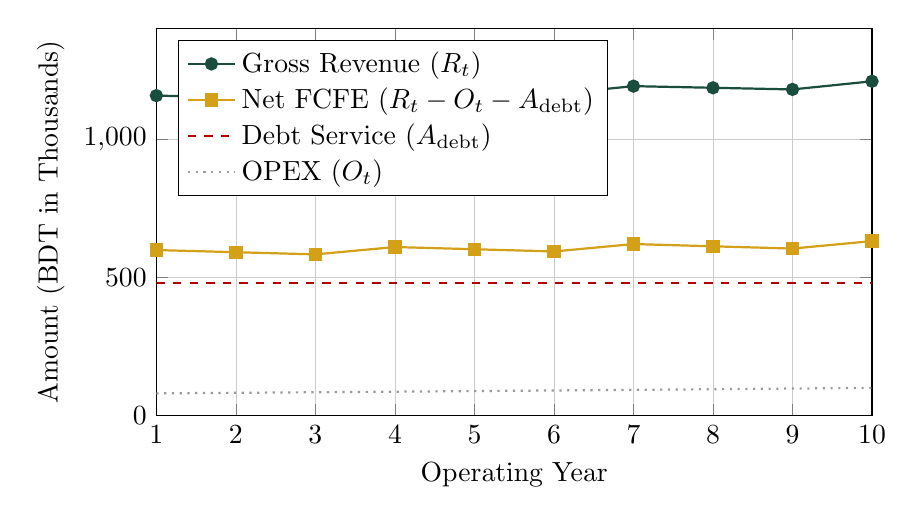
\begin{tikzpicture}
\begin{axis}[
    width=0.88\textwidth,
    height=6.5cm,
    xlabel={Operating Year},
    ylabel={Amount (BDT in Thousands)},
    xmin=1, xmax=10,
    ymin=0, ymax=1400,
    xtick={1,2,3,4,5,6,7,8,9,10},
    legend pos=north west,
    legend cell align={left},
    grid=both,
    grid style={line width=.1pt, draw=gray!20},
    major grid style={line width=.2pt,draw=gray!40},
]
\addplot[thick, color=netsogreen, mark=*] coordinates {
    (1, 1156.320) (2, 1150.538) (3, 1144.786) (4, 1173.348)
    (5, 1167.481) (6, 1161.644) (7, 1190.627) (8, 1184.674)
    (9, 1178.750) (10, 1208.163)
};
\addlegendentry{Gross Revenue ($R_t$)}

\addplot[thick, color=netsogold, mark=square*] coordinates {
    (1, 598.065) (2, 590.283) (3, 582.476) (4, 608.988)
    (5, 601.011) (6, 593.003) (7, 619.816) (8, 611.643)
    (9, 603.440) (10, 630.523)
};
\addlegendentry{Net FCFE ($R_t - O_t - A_{\text{debt}}$)}

\addplot[thick, color=red!70!black, dashed] coordinates {
    (1, 478.255) (2, 478.255) (3, 478.255) (4, 478.255)
    (5, 478.255) (6, 478.255) (7, 478.255) (8, 478.255)
    (9, 478.255) (10, 478.255)
};
\addlegendentry{Debt Service ($A_{\text{debt}}$)}

\addplot[thick, color=gray!80, dotted] coordinates {
    (1, 80.000) (2, 82.000) (3, 84.050) (4, 86.151)
    (5, 88.305) (6, 90.513) (7, 92.775) (8, 95.095)
    (9, 97.472) (10, 99.909)
};
\addlegendentry{OPEX ($O_t$)}
\end{axis}
\end{tikzpicture}
\caption{Ten-year financial cash flow projection for the Netso Energy 80~kWp CGS reference project under baseline debt terms (Scenario A), demonstrating EBITDA stability and debt coverage.}
\label{fig:cashflow}
\end{figure}

\subsection{Beringia Revenue-Share Stress Testing}
Under the Beringia Energy pure revenue-share structure, Year-1 gross revenue of BDT~1,156,320 yields BDT~374,712 (35\%) to the capital provider and BDT~781,608 (65\%) to Netso Energy. Net of 100\% absorbed OPEX (BDT~80,000), Netso retains BDT~701,608 in Year-1 operating profit \cite{rsa_doc}.

Table~\ref{tab:stress_test} evaluates project sensitivity across operational and credit shock scenarios \cite{stress_test}.

\begin{table}[htbp]
\centering
\small
\caption{Beringia Revenue-Share Structure Sensitivity and Downside Stress Test}
\label{tab:stress_test}
\begin{tabular}{lp{6.2cm}rr}
\toprule
\textbf{Scenario} & \textbf{Mechanism \& Impact} & \textbf{Netso Profit (Yr 1)} & \textbf{Investor Return Impact} \\
\midrule
\textbf{Baseline} & 35\% gross revenue split; 15.0\% unlevered IRR hurdle & BDT 701,608 & Payback $\approx$ 17.6 years \\
\textbf{Revenue $-10\%$} & Generation deficit or tariff floor (BDT 9.00/kWh) & BDT 621,608 ($-11.4\%$) & Payback expands to 19.6 yrs \\
\textbf{OPEX $+50\%$} & OPEX increases to BDT 120,000/yr (Netso absorbed) & BDT 661,608 ($-5.7\%$) & Unaffected (Gross split) \\
\textbf{Year 5 Buyback} & Early buyout exercised at 1.2$\times$ remaining unrecovered value & N/A & Target exit at BDT 5.67M \\
\textbf{Default Year 3} & CGS payment default; 6-mo bank guarantee + escrow drawn & Asset retained & Net loss capped at BDT 546k \\
\bottomrule
\end{tabular}
\end{table}

\section{Discussion}
\subsection{Structural Advantages of the True Variable Rate Method}
Conventional solar developers in Bangladesh frequently calculate savings estimates against blended electricity rates ($R_{\text{blend}} \approx \text{BDT } 14.81\text{/kWh}$), which incorrectly incorporate fixed maximum demand charges. Because fixed demand charges persist irrespective of distributed generation, projecting savings against blended figures overstates customer economic benefits. Netso Energy's methodology isolates the pure variable component ($R_{\text{var}} = \text{BDT } 12.98\text{/kWh}$), establishing an auditable 23.0\% cost reduction that withstands institutional scrutiny \cite{gt_constants, netso_venture}.

\subsection{Policy Upside and Capital Optimization}
The statutory exemptions in the FY2026--27 National Budget reducing clean energy component import tariffs to 0\% provide substantial upside for distributed infrastructure \cite{gt_constants}. Under Scenario~B, CAPEX declines from BDT~55,000/kW to BDT~40,000/kW. Rather than adjusting PPA tariffs downward, retaining the contract rate at BDT~10.00/kWh increases project DSCR from 2.25$\times$ to 3.09$\times$ and elevates levered equity IRR from 68.7\% to 114.1\%, enabling rapid capital recycling across pipeline facilities \cite{gt_constants}.

\subsection{Contractual Governance and Risk Mitigation}
In the Beringia revenue-share model, counterparty and structural risks are mitigated through four primary covenants:
\begin{enumerate}
    \item \textbf{Conditions Precedent:} Execution requires grid sanction load verification ($\ge 80\text{ kW}$ under the updated SREDA Net Metering Guidelines 2025 allowing up to 100\% of sanctioned load, improved from the previous 70\% ceiling that required $\ge 115\text{ kW}$) and Chattogram Development Authority (CDA) rooftop structural engineering certification \cite{rsa_doc}.
    \item \textbf{Payment Security:} Direct PPA billing flows into an irrevocable escrow account with an active 6-month first-demand bank guarantee (BDT~578,000) \cite{rsa_doc}.
    \item \textbf{Downside Preservation:} In the event of client default, modular pergola infrastructure can be unbolted and redeployed to alternative commercial properties \cite{stress_test}.
    \item \textbf{Arbitration Seat:} Legal disputes are bound exclusively to the Bangladesh Arbitration Act 2001 with legal seat in Dhaka \cite{rsa_doc}.
\end{enumerate}

\section{Conclusion}
This study validates the commercial, physical, and financial model of Netso Energy's 80~kWp reference solar pergola installation at CGS Chattogram. By coupling modular rooftop structural engineering with conservative variable tariff arbitrage (BDT~10.00/kWh PPA vs. BDT~12.98/kWh grid variable), the project delivers 23.0\% recurring savings to the client while producing robust debt service coverage (2.25$\times$) and high levered equity returns (68.7\% IRR). Non-dilutive revenue-share instruments offer an effective institutional bridge for early portfolio scale prior to long-term concessional debt refinancing.

\section*{References}
\begin{thebibliography}{9}
\bibitem{gt_constants} Netso Energy, ``Ground Truth Constants: Core Project Economics Specification,'' Internal Artifact \texttt{GROUND\_TRUTH\_CONSTANTS.md}, generated via \texttt{core\_economics.py}, Jun. 2026.
\bibitem{gt_financials} Netso Energy, ``Ground Truth Financials: Executable Financial Baseline for CGS Project,'' Knowledge Base Concept \texttt{concepts/ground-truth-financials.md}, Jul. 2026.
\bibitem{netso_product} Netso Energy, ``Product Specification and Platform Architecture,'' Documentation Artifact \texttt{PRODUCT.md}, Netso Energy Repository, Jul. 2026.
\bibitem{netso_entity} Netso Energy, ``Venture Entity Overview and Operating Metrics,'' Knowledge Base Entity \texttt{entities/netso-energy.md}, Jul. 2026.
\bibitem{beringia_entity} Beringia Energy Global LLC / Beringia Power Bangladesh, ``Capital Partner Profile and Transaction Terms,'' Knowledge Base Entity \texttt{entities/beringia-energy.md}, Jul. 2026.
\bibitem{rsa_doc} Netso Energy and Beringia Power Bangladesh, ``Revenue Share Agreement: CGS 80kW Solar Facility Financing Terms,'' Knowledge Base Concept \texttt{concepts/revenue-share-agreement.md}, Jul. 2026.
\bibitem{stress_test} Netso Energy, ``Beringia Revenue Share Structure Sensitivity and Downside Stress Test,'' Knowledge Base Concept \texttt{concepts/beringia-stress-test.md}, Jul. 2026.
\bibitem{solar_ppa} Netso Energy, ``Solar PPA Commercial Model and Net Metering Interface,'' Knowledge Base Concept \texttt{concepts/solar-ppa-model.md}, Jul. 2026.
\bibitem{netso_venture} TAZ OS, ``Venture Instance Specification: Netso Energy (VEN-NETSO-001),'' Configuration File \texttt{raw/articles/netso-venture.yml.md}, Jun. 2026.
\end{thebibliography}

\end{document}
